% Compact PGFPlots panel for sampled qldpc_20_2_4_signature_cap4 BSC correction-class derivative.
% Requires \usepackage{pgfplots} and \pgfplotsset{compat=1.18}.
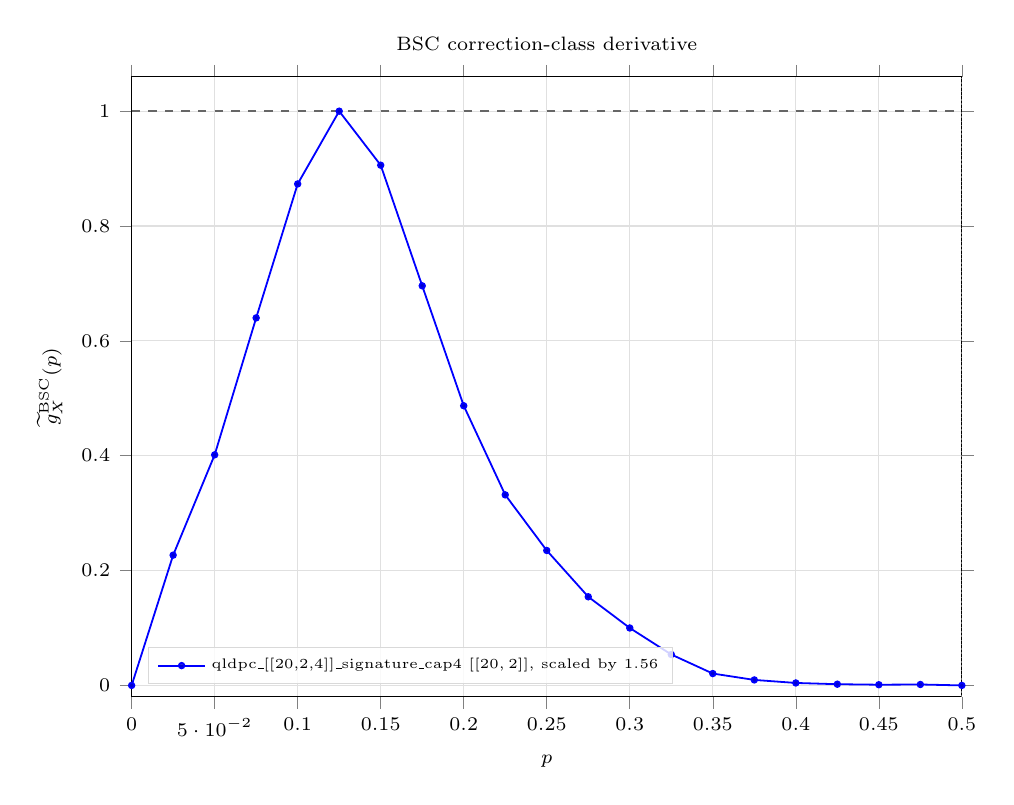
\begin{tikzpicture}
\begin{axis}[
  name=scaledBSCGEXITQldpc2024SignatureCap4Axis,
  width=\linewidth,
  height=0.78\linewidth,
  title={BSC correction-class derivative},
  title style={font=\scriptsize},
  xlabel={$p$},
  ylabel={$\widetilde g_X^{\rm BSC}(p)$},
  xmin=0, xmax=0.5,
  ymin=-0.02, ymax=1.06,
  grid=both,
  major grid style={black!12},
  minor grid style={black!6},
  tick align=outside,
  tick label style={font=\scriptsize},
  label style={font=\scriptsize},
  legend cell align={left},
  legend style={draw=black!15, fill=white, fill opacity=0.82, text opacity=1, at={(0.02,0.02)}, anchor=south west, font=\tiny},
]
\addplot[black!60, densely dotted, line width=0.55pt, forget plot] coordinates {(0.5,-0.02) (0.5,1.06)};
\addplot[black!60, dashed, line width=0.55pt, forget plot] coordinates {(0,1) (0.5,1)};
\addplot+[color=blue, mark=*, mark size=1.0pt, line width=0.65pt]
coordinates {(0,0) (0.025,0.226887701309) (0.05,0.401514649187) (0.075,0.640022884706) (0.1,0.873331986175) (0.125,1) (0.15,0.90593676328) (0.175,0.695869659995) (0.2,0.486997951334) (0.225,0.331835919639) (0.25,0.235010592052) (0.275,0.154383061905) (0.3,0.100030880852) (0.325,0.053849393643) (0.35,0.0206602649509) (0.375,0.0095824555502) (0.4,0.00429861469365) (0.425,0.00211491579884) (0.45,0.00121766518742) (0.475,0.0016206831813) (0.5,0)};
\addlegendentry{qldpc\_[[20,2,4]]\_signature\_cap4 $[[20,2]]$, scaled by $1.56$}
\end{axis}
\end{tikzpicture}
